% Chapter 5

\chapter{Results} % Main chapter title

\label{results} % For referencing the chapter elsewhere, use \ref{Chapter1} 

\lhead{Chapter 6. \emph{Results and Discussion}} % This is for the header on each page - perhaps a shortened title

%----------------------------------------------------------------------------------------

\section{Drag and lift on a cylinder}
The effect of the algorithm explained in Chapter~\ref{xyzarc} is
illustrated by solving a laminar flow test problem. 
The solution is compared with previously benchmark computations performed by a number of 
contributors~\cite{benchmark}. 

The results can be found in 
table~\ref{tab:testcase}. As the results clearly show the treatment of the geometry is 
crucial, both coefficients are computed with significantly better accuracy. 
%
\begin{table}
\centering
\begin{tabular}{l l c c c c}
		\toprule
		\# of Cells & Software & $c_D$ & $c_L$ & \%\textbf{Err} $c_D$ &\%\textbf{Err} $c_L$ \\ \midrule 
		2070 & Nek5000 (mid) & 6.18349 & 0.008939 & 0.030 & 4.19 \\ 
		2070 & Nek5000 (arc) & 6.18498 & 0.009413 & 0.006 & 0.13 \\
		3145728 & CFX 		 & 6.18287 & 0.009387 & 0.04 &0.15 \\
		3145728 & OF	     & 6.18931 & 0.00973 & 0.06 &3.5 \\
		3145728 & FEATFLOW   & 6.18465 & 0.009397 & 0.01 &0.05 \\
		\bottomrule	
	\end{tabular}
	\caption{Results for the drag and lift coefficients with reference values 
	$c_D = 6.18533$ and $c_L = 0.009401$.}
\label{tab:testcase}
\end{table}
%
The polynomial degree used in the calculations with Nek5000 was chosen as $p = 11 $ 
in all directions. The explicit number of cells is therefore $2070\cdot11^{3} = 2755170$,
approximately $88\%$ of the number of cells used for the benchmark simulations. Compared 
with the results from the other softwares applied in~\cite{benchmark} Nek5000 performs 
just as well or better in most cases. It should be mentioned that the division of the grid is done 
differently for Nek5000 so the comparison is not as direct as it may seem from the table.


\colorbox{yellow}{add more info about the mesh for this case??}

\subsection{Parameter adjustments in Nek5000}
As discussed in chapter~\ref{nek} there are many adjustments available in Nek. 
In order to enlighten the actual effect on the results, several different settings have 
been investigated and the results are presented in table~\ref{tab:perf}. The spectral convergence
is also confirmed in figure~\ref{fig:liftconv}. 
%
\begin{figure}[h]
	\centerline{
        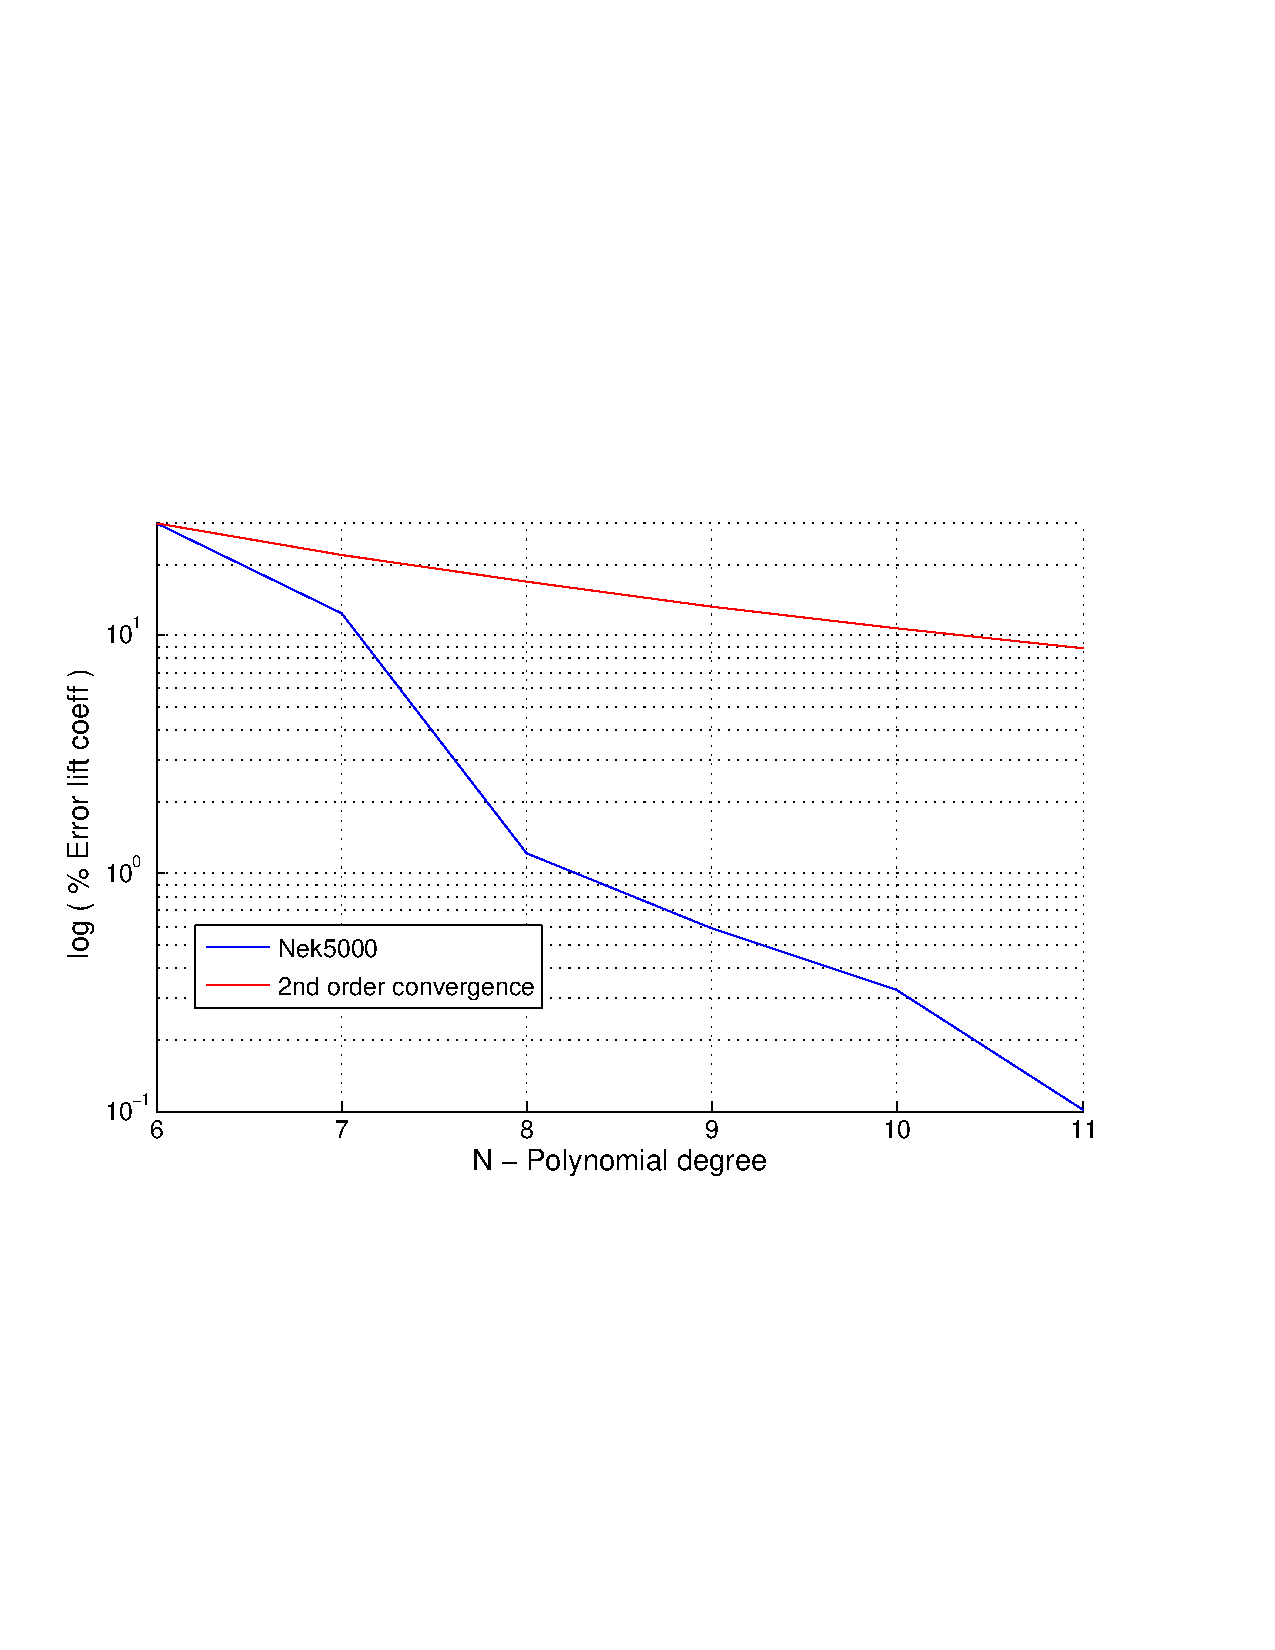
\includegraphics[trim=0.5cm 7cm 0.5cm 7cm, width=0.8\textwidth]{Figures/lift_coef2.pdf}}
	\caption{The logarithm of the error plotted against the polynomial degree. All results 
        are with $P_nP_{n-2}$ and dealiasing, and they are solved without using the 
    characteristic scheme or any filtering.}
	\label{fig:liftconv}
\end{figure}
%

The settings that sticks out in this test is the $P_nP_n$ scheme which clearly performs 
worse than the others. This is as expected because of the splitting scheme applied, which 
induces nonvanishing errors in the pressure close to the boundary.
Use of the IOFS method also has a negative effect on the accuracy, at least for the lift coefficient,
this is also as expected because of its stability properties, it is important to mention that with 
this scheme a much higher time step is allowed. The filtering is the least significant change
which confirms the analytical results from~\ref{eq:filterenergy}. The effect is suspected to 
increase if the same test was performed for a smaller $N$.
%
\begin{table}[h]
    \centering
    \begin{tabular}{c | c c c c | c c }
         & \multicolumn{4}{|c|}{Settings} & \multicolumn{2}{|c|}{\% Error} \\\hline
         \#  & ifsplit & Dealiasing & IOFS & Filter & $c_D$ & $c_L$ &  \hline 
         1 & F & T & F & F & 0.005 & 0.102 \\
         2 & T & T & F & F & 0.013 & 2.349 \\
         3 & F & T & F & T & 0.005 & 0.431 \\
         4 & F & T & T & F & 0.005 & 0.179 \\
         5 & F & F & F & F & NaN   & NaN   \\
    \end{tabular}
    %\begin{tabular}{c | c c c c | c c | c c c}
         %& \multicolumn{4}{|c|}{Settings} & \multicolumn{2}{|c|}{\% Error} & \multicolumn{3}{|c}{Data} \\\hline
         %\#  & ifsplit & Dealiasing & IOFS & Filter & $c_D$ & $c_L$ & DT & CFL & T/Tstep \\ \hline 
         %1 & F & T & F & F & 0.005 & 0.102 & 1e-04 & 2.03 & 2.1e-02 \\
         %2 & T & T & F & F & 0.013 & 2.349 & 1e-04 & 2.03 & 2.1e-02 \\
         %3 & F & T & F & T & 0.005 & 0.431 & 1e-04 & 2.03 & 2.1e-02 \\
         %4 & F & T & T & F & 0.005 & 0.179 & 1e-04 & 2.03 & 2.1e-02 \\
         %5 & F & F & F & F & NaN   & NaN   & 1e-04 & 2.03 & 2.1e-02 \\
    %\end{tabular}
    \caption{Test of solver settings in Nek5000}
    \label{tab:perf}
\end{table}
%

Be aware that these results are obtained from a laminar test case and does not in any way 
suggest any optimal adjustment for Nek5000. The results are included to gain a better understanding
of how the different settings can affect the solution.

%----------------------------------------------------------------------------------------
\section{Gas dispersion in a simplified urban area} 
This case is a part of a larger project designed to evaluate different solvers 
ability to perform simulations of gas dispersion. The N-S equations are solved using
the $P_nP_n$ formulation with the fractional step method, IOFS with a target Courant number 
equal 2 was enabled to maximize the time step as recommended in~\cite{Nek}. It should be 
mentioned that the stability properties when activating the SGS-model and deactivating the 
filtering was greatly reduced. This effect is captured in~\ref{fig:maxvel} which shows how 
spurious velocity modes are not dampened in the same degree as with the Smagorinsky model. 

An initial attempt to simulate the 
dispersion of gas was performed in Nek5000 with fairly coarse element sizes, but without
any subgrid-scale model. Only applying filtering on the last 3 modes made the solution 
sufficiently stable and the results together with the Smagorinsky model can be seen in figures~\ref{fig:cHfilter} and~\ref{fig:cHfilter}.
%
\begin{figure}[h]
	\centering
	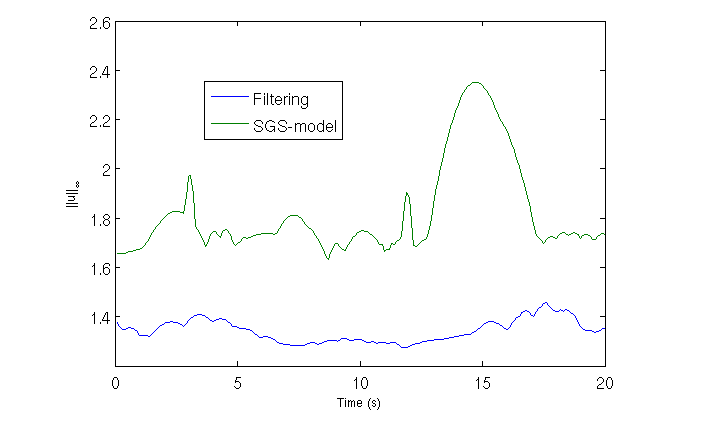
\includegraphics[width=0.6\textwidth]{Figures/maxvel.png}
	\caption{A average iso-surface of the released gas at $C=0.03$ 
    after 30 seconds of sampling.}
	\label{fig:maxvel}
\end{figure}
%
%
\begin{figure}[h]
	\centering
	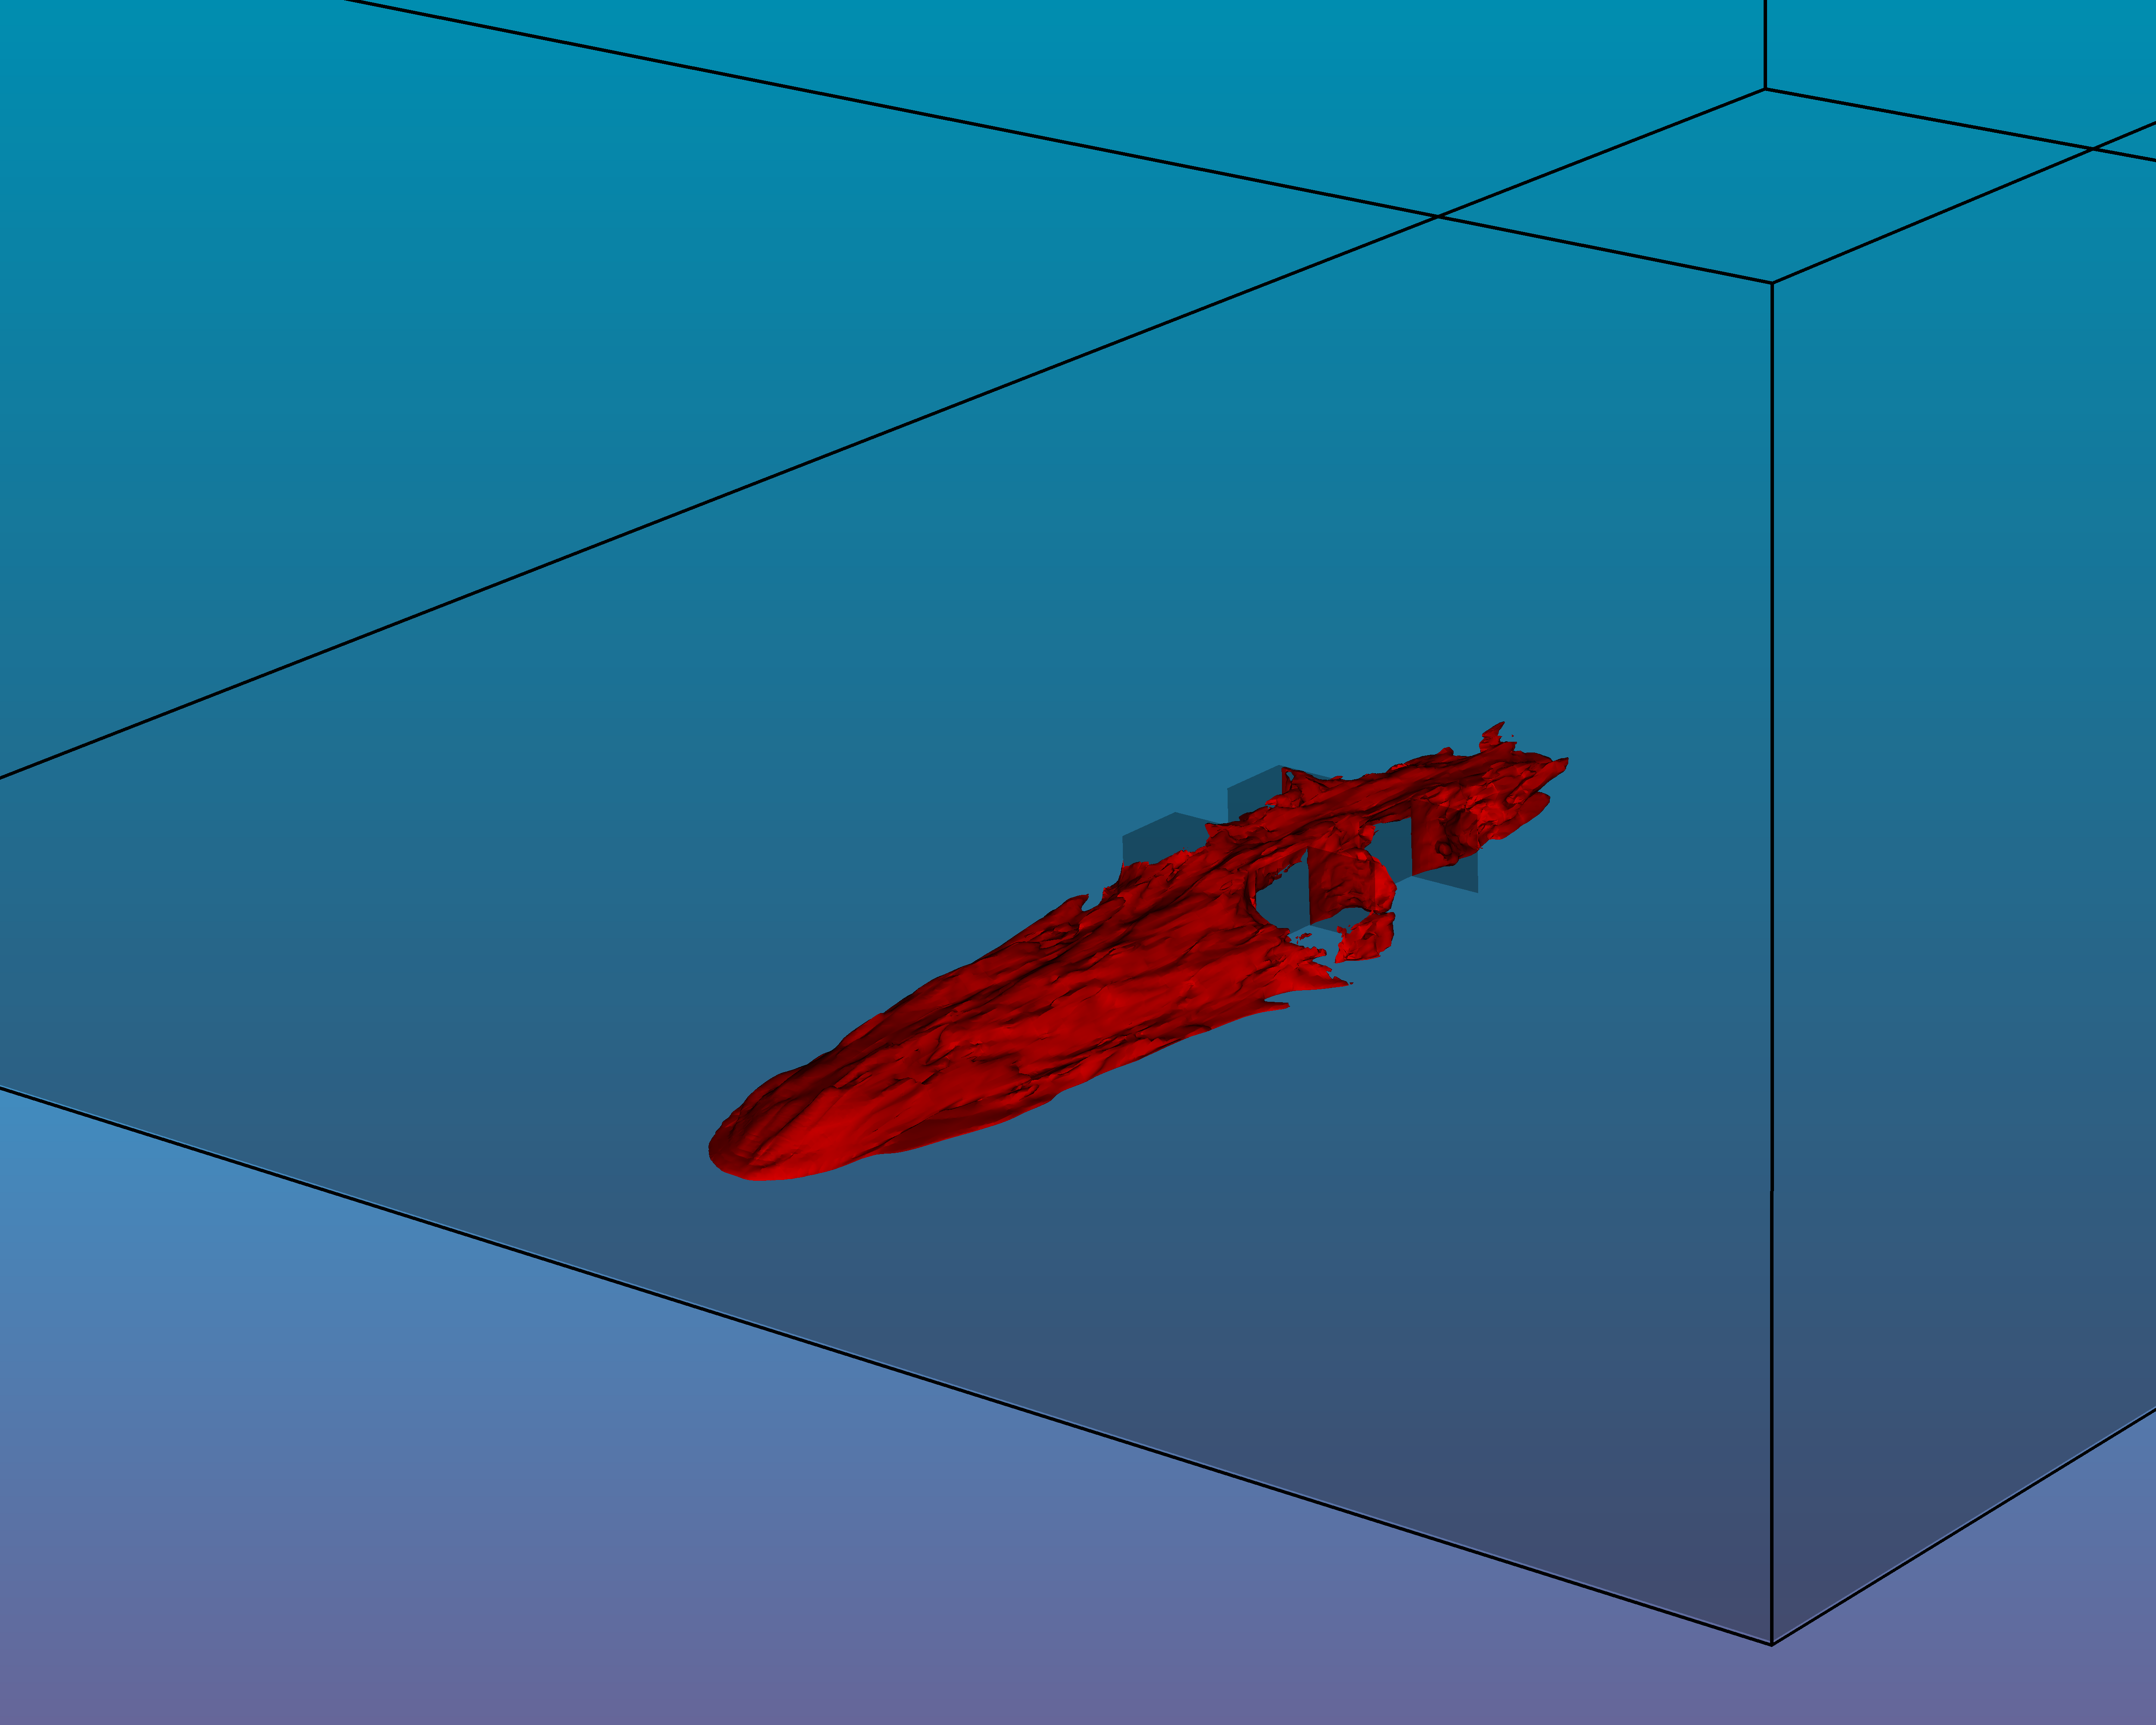
\includegraphics[width=0.6\textwidth]{Figures/plume.png}
	\caption{A average iso-surface of the released gas at $C=0.03$ 
    after 30 seconds of sampling.}
	\label{fig:plume}
\end{figure}
%
%
\begin{figure}[h]
	\centering
	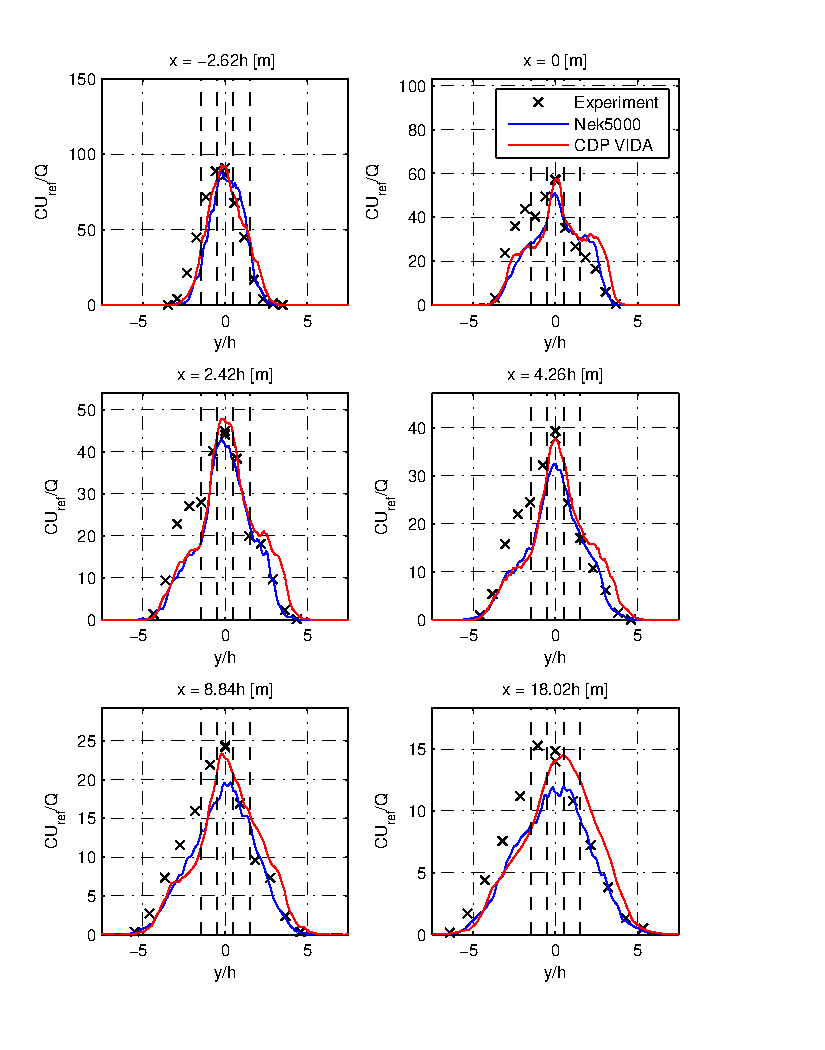
\includegraphics[width=0.8\textwidth]{Figures/NekcH.pdf}
	\caption{Time-averaged concentration with a sample time of $18.00$ s at $z/H = 0.025$ plotted horizontally and scaled 
	with the free-stream velocity and emission rate. Compared against wind tunnel data.
Two dashed lines on either side of the centerline represent the canyon.}
	\label{fig:cHfilter}
\end{figure}
%
Discuss the plot... 

%
\begin{figure}[h]
	\centerline{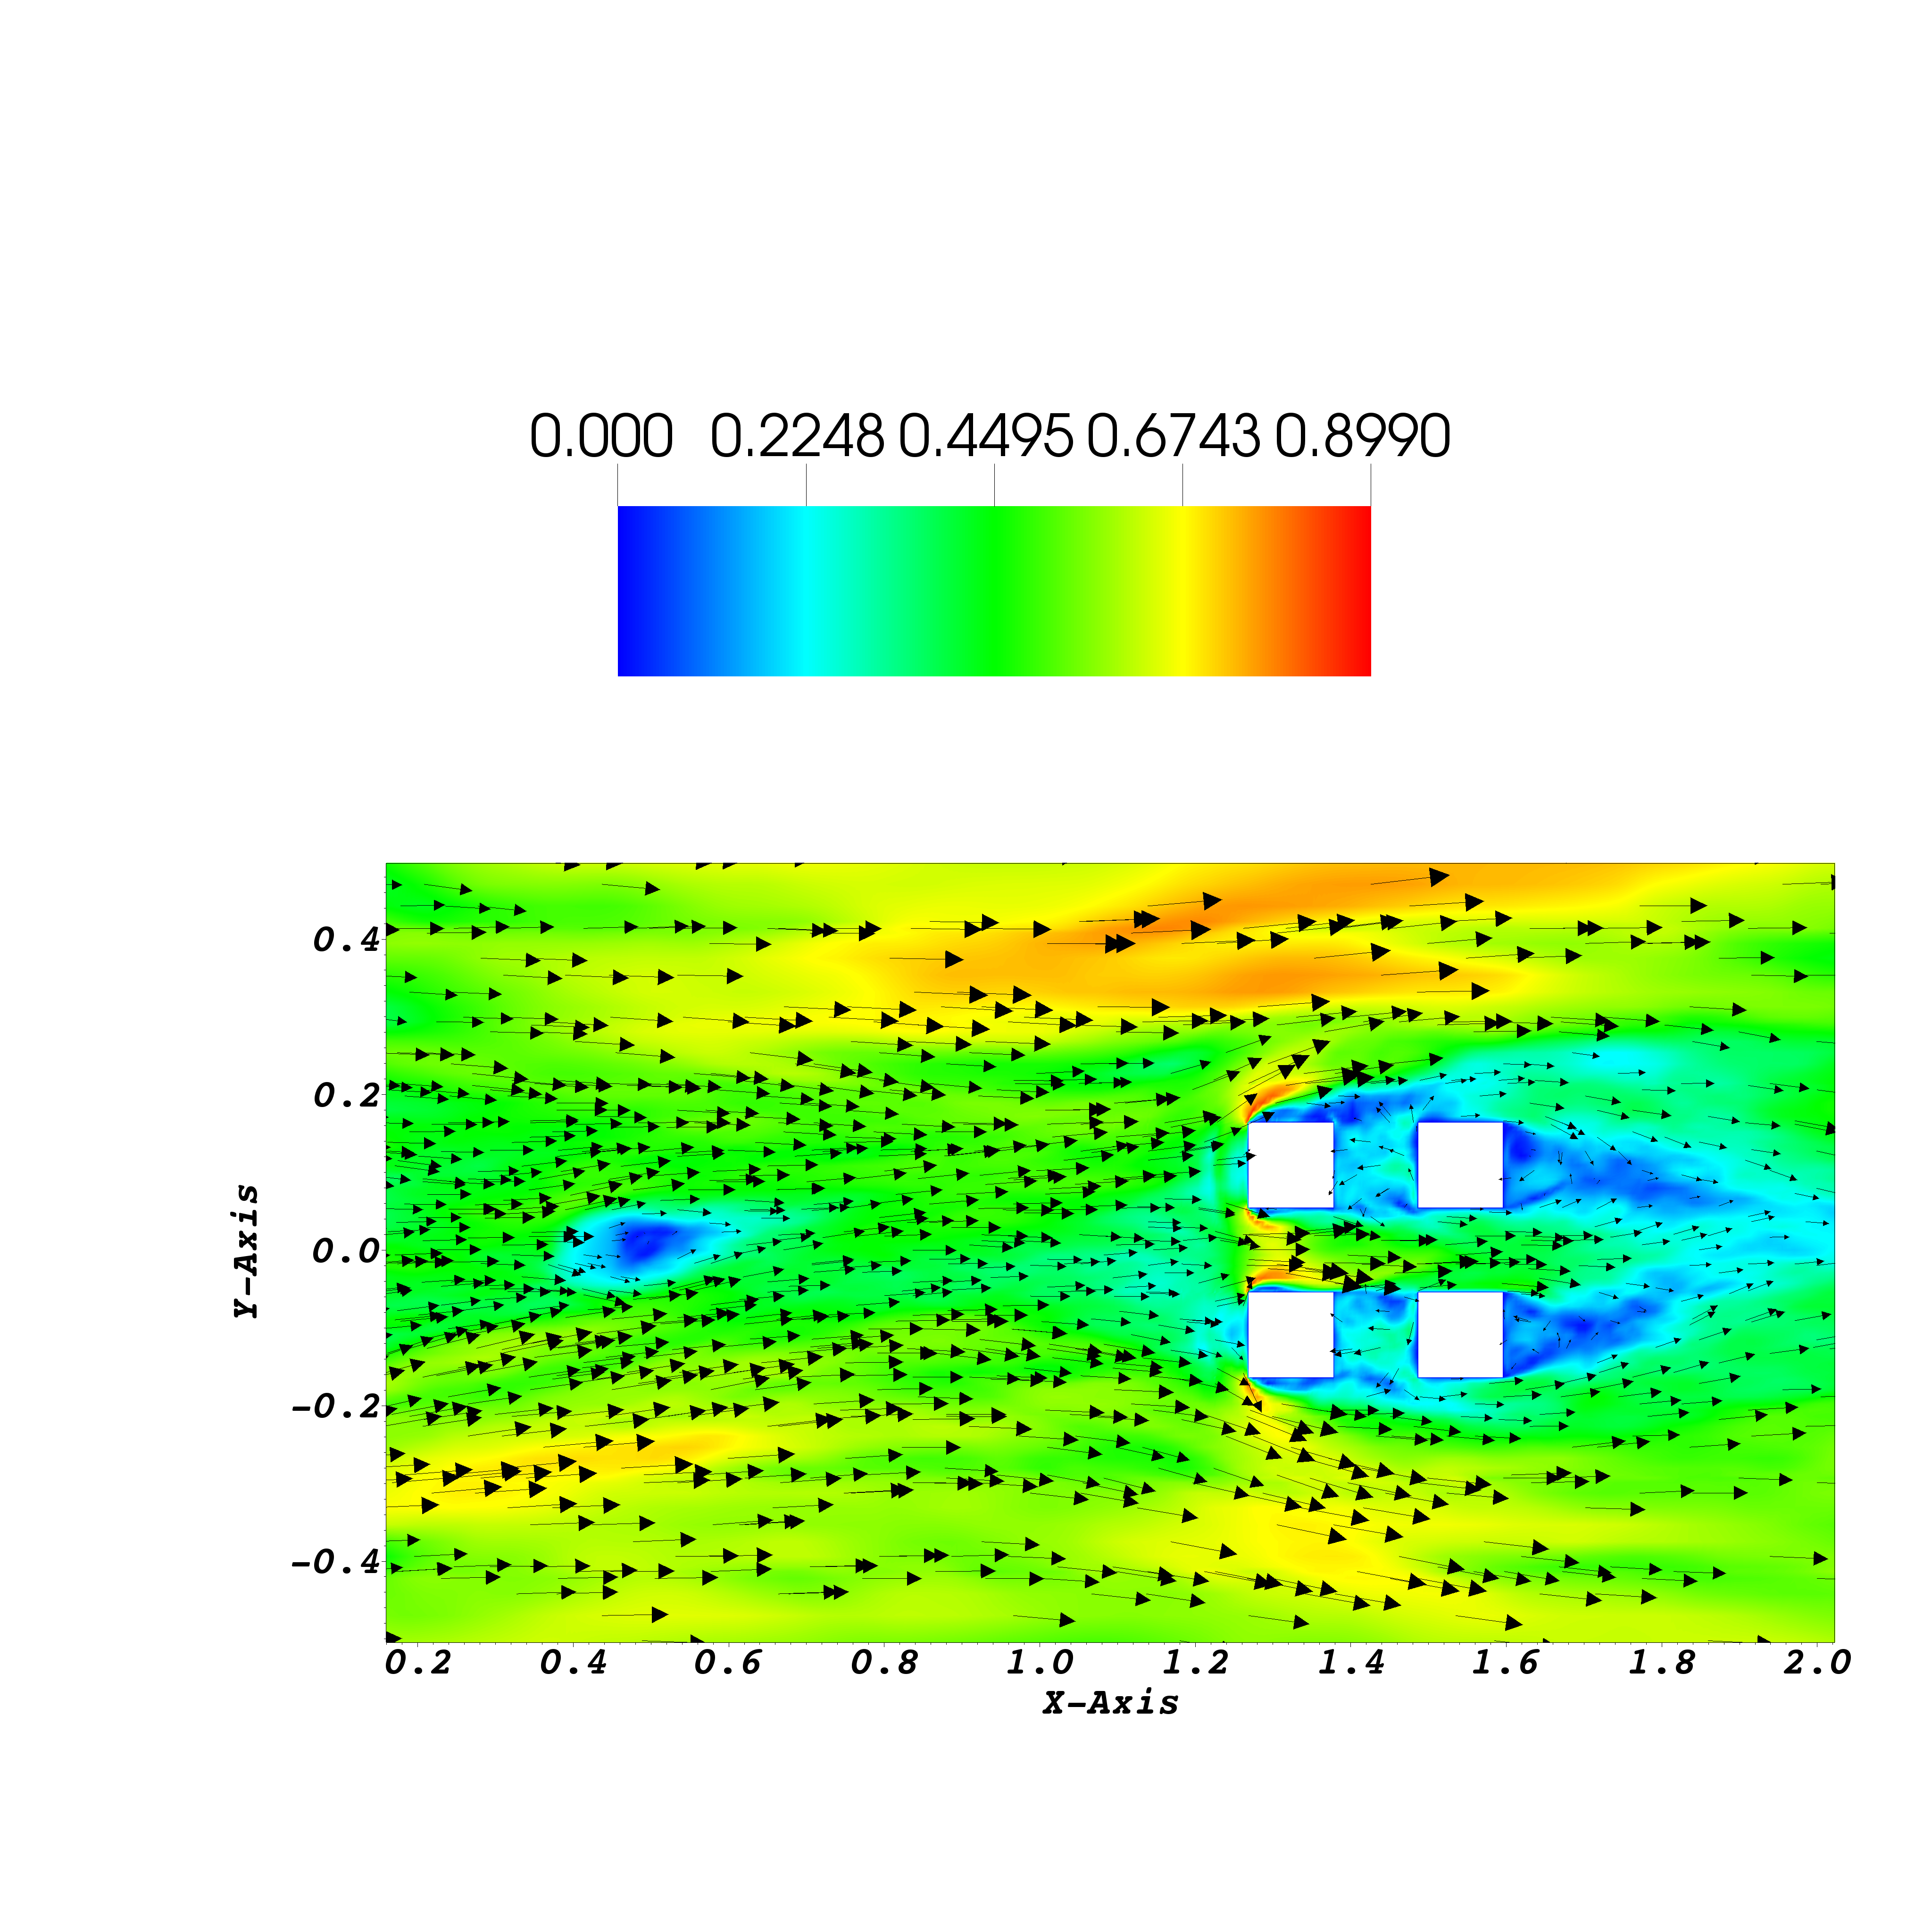
\includegraphics[width=0.8\textwidth]{Figures/vel_field.png}}
	\caption{velocity field for $z= 0.02$m, around the source and the cubes.}
	\label{fig:vel_field}
\end{figure}
%

\colorbox{green}{redo these simulation in case they were started to early.}
%
%\begin{figure}[h]
	%\centering
	%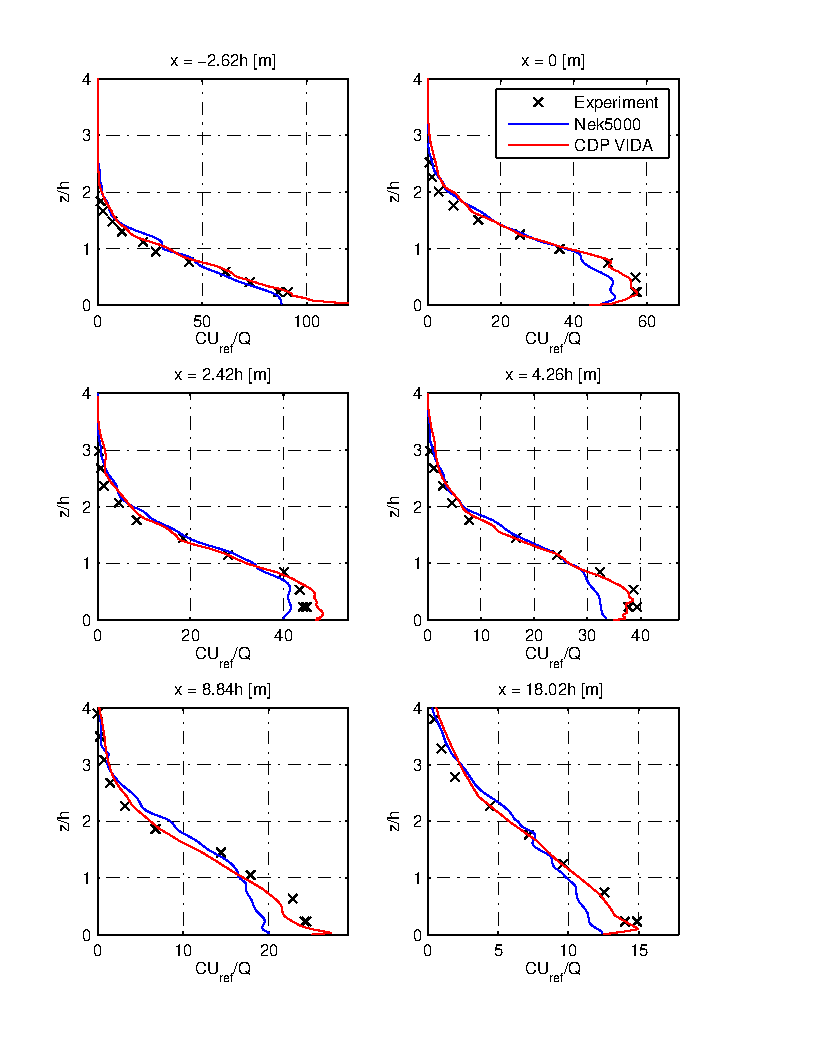
\includegraphics[width=0.8\textwidth]{Figures/NekcV.pdf}
	%\caption{Time-averaged concentration with a sample time of $18.00$ s at $y = 0$ plotted
    %vertically and scaled 
	%with the free-stream velocity and emission rate. Compared against wind tunnel data.
%Two dashed lines on either side of the centerline represent the canyon.}
	%\label{fig:cVfilter}
%\end{figure}
%
%
\begin{figure}[h]
	\centering
	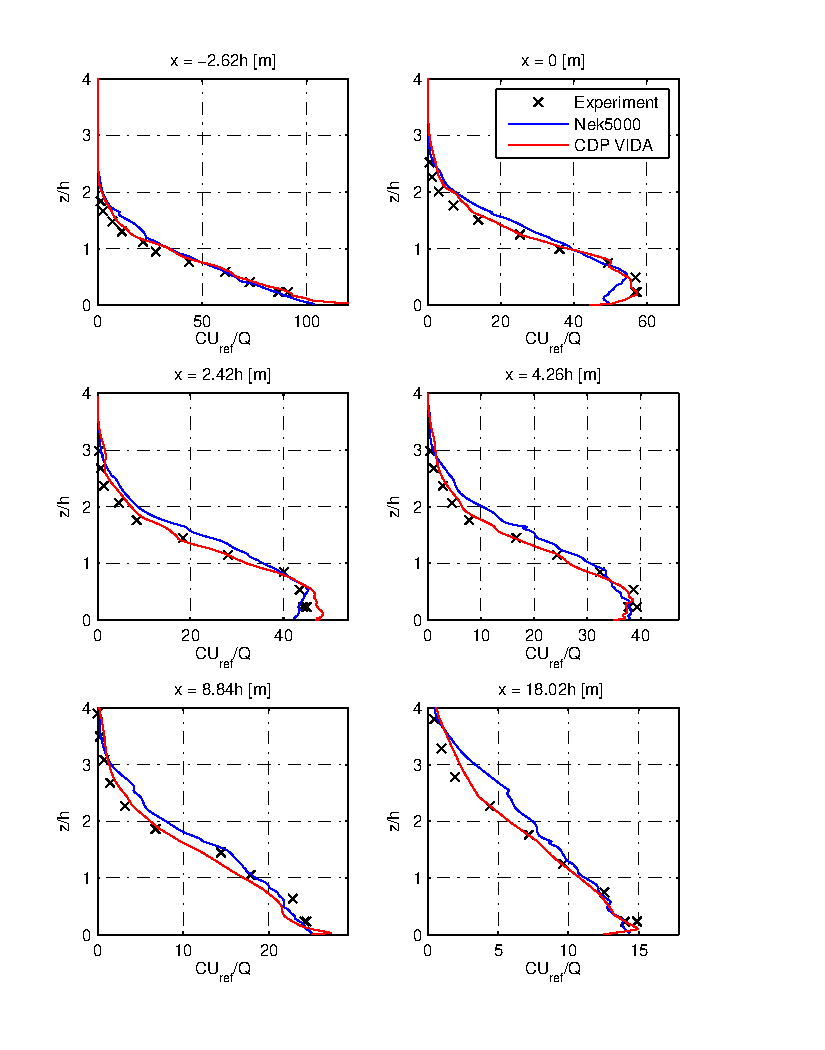
\includegraphics[width=0.8\textwidth]{Figures/Nek_smag_cV.pdf}
	\caption{Time-averaged concentration with a sample time of $22.00$ s at $y = 0$ plotted
    vertically and scaled 
	with the free-stream velocity and emission rate. Compared against wind tunnel data.
Two dashed lines on either side of the centerline represent the canyon.}
	\label{fig:cVsmag}
\end{figure}
%
%
\begin{figure}[h]
	\centering
	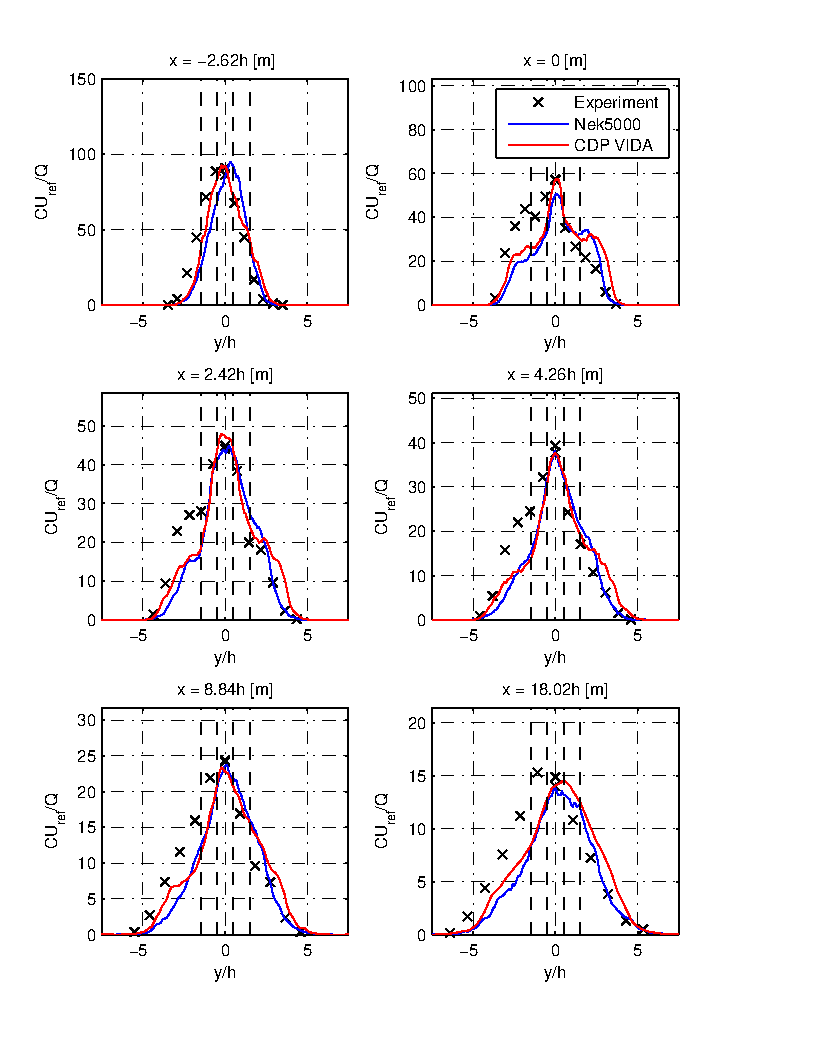
\includegraphics[width=0.8\textwidth]{Figures/Nek_smag_cH.pdf}
	\caption{Time-averaged concentration with a sample time of $22.00$ s at $y = 0$ plotted
    vertically and scaled 
	with the free-stream velocity and emission rate. Compared against wind tunnel data.
Two dashed lines on either side of the centerline represent the canyon.}
	\label{fig:cVsmag}
\end{figure}
%


%\begin{figure}[h]
    %\centering
    %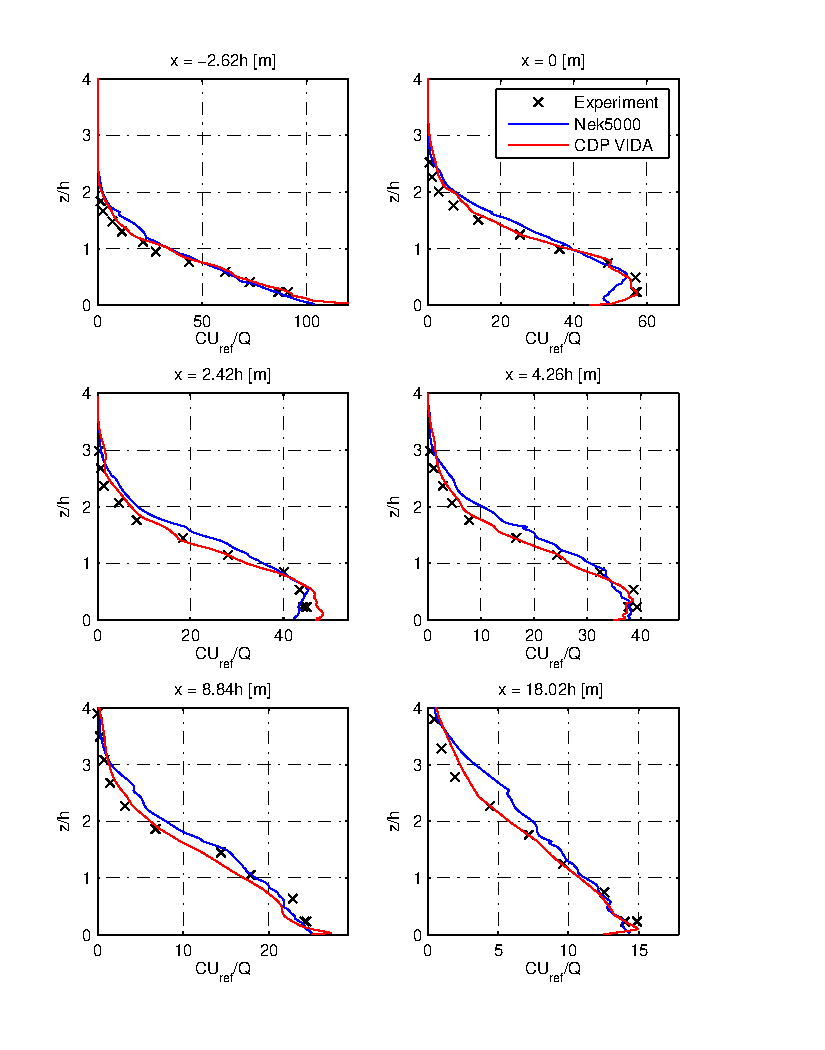
\includegraphics[width=0.8\textwidth]{Figures/Nek_smag_cV.pdf}
    %\caption{Time-averaged concentration with a sample time of $22.00$ s at $y = 0$ plotted
    %vertically and scaled 
    %with the free-stream velocity and emission rate. Compared against wind tunnel data.
%Two dashed lines on either side of the centerline represent the canyon.}
    %\label{fig:cVsmag}
%\end{figure}


%\begin{figure}[h]
    %\centering
    %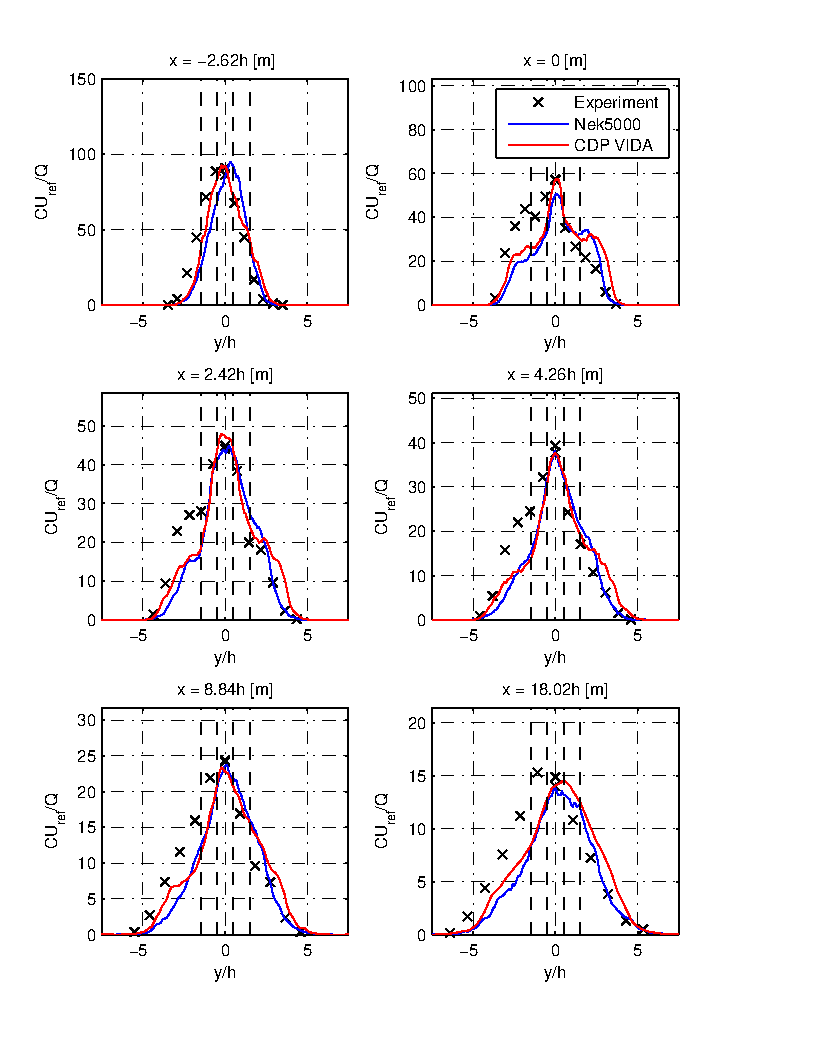
\includegraphics[width=0.8\textwidth]{Figures/Nek_smag_cH.pdf}
    %\caption{Time-averaged concentration with a sample time of $22.00$ s at $y = 0$ plotted
    %vertically and scaled 
    %with the free-stream velocity and emission rate. Compared against wind tunnel data.
%Two dashed lines on either side of the centerline represent the canyon.}
    %\label{fig:cVsmag}
%\end{figure}


%\begin{figure}[h]
    %\centering
    %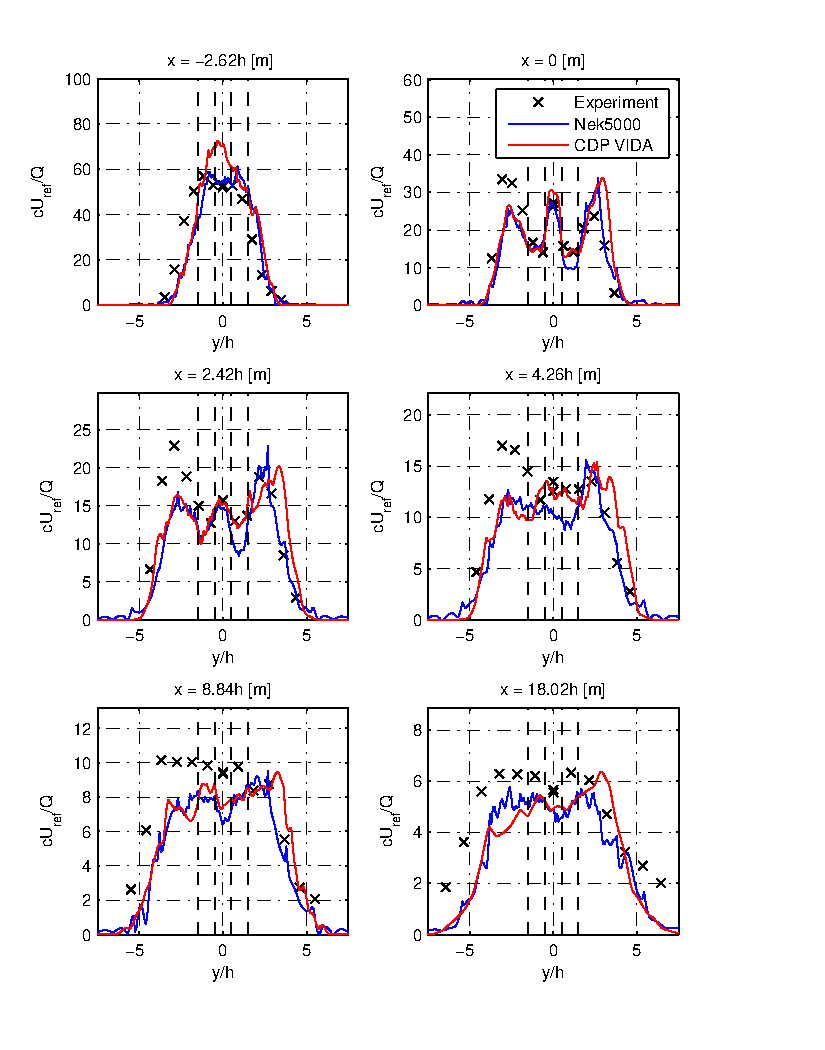
\includegraphics[width=0.8\textwidth]{Figures/Nek_smag_cfluctH.pdf}
    %\caption{Time-averaged concentration with a sample time of $22.00$ s at $y = 0$ plotted
    %vertically and scaled 
    %with the free-stream velocity and emission rate. Compared against wind tunnel data.
%Two dashed lines on either side of the centerline represent the canyon.}
    %\label{fig:cVsmag}
%\end{figure}


\section{Discussion and Conclusion}
\colorbox{green}{How did Nek perform overall, user-friendly ?,correctness,speed etc.}

